\documentclass[11pt,a4paper]{article}
% Built from docs/manuscript/manuscript.md (export of the Claude Doc) by a one-off script.
\usepackage[margin=25mm]{geometry}
\ifdefined\XeTeXversion
  \usepackage{fontspec}
\else
  \usepackage[utf8]{inputenc}
  \usepackage[T1]{fontenc}
  \usepackage{lmodern}
  \usepackage{textcomp}
\fi
\usepackage{amsmath,amssymb}
\usepackage{graphicx}
\usepackage{longtable,booktabs,array,calc}
\usepackage{pdflscape}
\usepackage{etoolbox}
\usepackage{xcolor}
\usepackage[hidelinks]{hyperref}
\urlstyle{same}
\usepackage{microtype}
\setlength{\parskip}{4pt plus 1pt}
\setlength{\emergencystretch}{3em}
\providecommand{\tightlist}{\setlength{\itemsep}{0pt}\setlength{\parskip}{0pt}}
\AtBeginEnvironment{longtable}{\footnotesize}
\makeatletter
\newsavebox\pandoc@box
\newcommand*\pandocbounded[1]{%
  \sbox\pandoc@box{#1}%
  \Gscale@div\@tempa{\textheight}{\dimexpr\ht\pandoc@box+\dp\pandoc@box\relax}%
  \Gscale@div\@tempb{\linewidth}{\wd\pandoc@box}%
  \ifdim\@tempb\p@<\@tempa\p@\let\@tempa\@tempb\fi
  \ifdim\@tempa\p@<\p@\scalebox{\@tempa}{\usebox\pandoc@box}%
  \else\usebox{\pandoc@box}%
  \fi%
}
\makeatother
\graphicspath{{./}}

\title{DataBaseAgent: a local desktop workbench for building topic-specific
biological data repositories with human-gated AI agents}
\author{Zhougeng Xu \textsuperscript{1,*}, {[}co-author placeholders{]}\\[2pt]
\textsuperscript{1} {[}institution, city, country{]}\\[2pt]
{[}email{]}}
\date{Draft of 5 November 2026}

\begin{document}
\maketitle

\begin{abstract}
Agent-curated repositories such as scBaseCount show that large language
model (LLM) agents can discover, annotate and reprocess public
sequencing data at a scale manual curation cannot reach. That
demonstration is a single bespoke repository: its agent, pipeline and
cloud deployment were engineered for one assay by one institute. Most
researchers need something smaller and more specific, such as every
public dataset on their organism, tissue or perturbation of interest,
processed uniformly with tools they trust, and few have the engineering
capacity to build it; GPSAdb, a manually curated compendium of 3,048
human gene-perturbation RNA-seq datasets, is the authors' own instance
of that need. Here we present DataBaseAgent (DBA), a general-purpose
desktop workbench that turns the agent-curated repository pattern into a
tool any researcher can run. DBA ships as one binary for Windows, macOS
and Linux with no server or database to deploy. A project states its
topic, organism, assay and inclusion criteria in free text. Candidates
are gathered from Europe PMC, PubMed or GEO, or imported. An LLM
reviewer proposes include, exclude or uncertain with a verbatim evidence
snippet that the application verifies against the record; a dataset
enters the repository only through a recorded decision that carries a
written reason and names who made it. The user writes the processing
pipeline as ordinary shell steps and locks a version. Jobs run on the
user's own Linux server over SSH under CPU and concurrency quotas;
network failures are retried a bounded number of times and everything
else is escalated to the user with the log and a resume point. Outputs
are checksummed, manifested and archived locally. One project agent and
four specialists, each with its own model, instructions and fixed tool
list, work in a single conversation per project; they act only through
the same validated commands as the interface, run only when addressed,
and every call is recorded in the conversation. Any OpenAI-compatible,
Anthropic or Gemini endpoint, including locally served models, can be
the model. We present DBA as a design contribution: its workflow and
architecture, the safeguards around acting agents, two walkthroughs on
live services, one of which carries a single GPSAdb-style dataset from a
GEO search through a help request to a checksummed count matrix, and a
feature comparison with repository-scale curation agents, dataset
fetchers, screening tools and workflow platforms. Usability and the
quality of the repositories users build with it remain to be evaluated.
DBA is open source at {[}repository URL{]}.
\end{abstract}

{\small
\textbf{Keywords:} data curation, AI agents, human-in-the-loop,
reproducible pipelines, desktop software, sequencing data repositories

\textbf{Preprint status:} draft for bioRxiv (Bioinformatics). Software
name in the text: DataBaseAgent (DBA). Comparator named in the brief as
``ScBaseAgent'' is scBaseCount with its SRAgent curation agent
(Youngblut et al., Cell 2026); the draft uses the published names.

\textbf{Draft conventions:} square brackets mark placeholders the
authors must fill or confirm; every quantitative claim about DBA comes
from the repository (README, tests, acceptance record and single-dataset
case record of 5 November 2026, at commit 37104a6) and is cited to it;
nothing about runtime performance or user studies is claimed because
none has been measured.
}

\section{Introduction}\label{introduction}

Public sequencing archives hold far more data than any community uses.
The Sequence Read Archive (SRA) and the Gene Expression Omnibus (GEO)
grow faster than curated atlases can absorb them, and most of their
content is reachable only through free-text metadata that was written
for submission, not for reuse {[}2,3{]}. Uniformly reprocessed resources
such as ReCount and recount3, ARCHS4 and refine.bio showed that
re-running one pipeline over thousands of public experiments removes
processing artefacts and makes cross-study analysis routine {[}4,5,6{]}.
Each of them, however, is a centrally built product with a fixed scope,
and the labour of selecting, annotating and reprocessing datasets is
paid once by one team.

scBaseCount moved that labour to an AI agent {[}1{]}. Its curation
agent, SRAgent, is a hierarchy of ReAct-style language-model agents
{[}8{]} that queries NCBI tools, decides whether an SRA experiment is
10x Genomics single-cell data, extracts organism, tissue and disease,
and stores the result in a relational database; a Nextflow pipeline,
scRecounter, then reprocesses every accepted experiment {[}9{]}. The
outcome is the largest public single-cell repository, more than 502
million cells from 27 organisms, and the authors show that agentic
extraction recovers metadata that deterministic tools such as ffq and
pysradb cannot {[}1,16,17{]}. They also state the general lesson: the
approach ``provides a blueprint for how AI can be leveraged to
autonomously curate biological data repositories'' {[}1{]}. The
blueprint itself, though, is not something a typical laboratory can pick
up. SRAgent runs on Google Cloud Run against a hosted PostgreSQL
database, scRecounter runs on GCP Batch, the pipeline is specific to 10x
chemistry, and the published run consumed an estimated 13.2 trillion
tokens at a cost of about 17,000 USD {[}1{]}.

Most repository needs sit in the long tail below that scale, and the
authors' own database is the motivating case. GPSAdb collects human
cell-line RNA-seq datasets in which one gene was knocked out or down:
3,048 datasets for 1,458 genes in its published version, each found by
searching GEO and ENCODE with knockdown and knockout terms, screened by
hand, given its control and perturbed samples by hand, and reprocessed
with one pipeline into differential expression tables and 6,096 gene
sets that its GPSA tool uses to infer candidate causal perturbations
from a user's own expression data {[}32{]}. The paper promised an annual
survey of new data; the database registry lists its last update as
August 2022 {[}33{]}, because every update repeats the whole manual
cycle. Other groups face the same cycle: a plant group wants every
public single-cell dataset of a root tissue, a disease group every bulk
cohort that matches a phenotype, a perturbation group every screen that
targeted a pathway. Today such a group stitches together a search in
PubMed or Europe PMC, a spreadsheet of candidates, a fetching tool such
as pysradb, ffq or nf-core/fetchngs {[}15,16,17{]}, a workflow manager
{[}9,10,25{]}, and a cluster account, and then keeps the whole
arrangement alive by hand. Platforms such as Galaxy and Seqera cover
execution well but start after the datasets have been chosen {[}11{]};
screening tools such as ASReview and Rayyan triage literature but stop
before any data is touched {[}14,23{]}; and general-purpose biomedical
agents such as Biomni and CellAgent analyse data already in hand without
addressing which datasets to gather {[}13,22{]}. Building the repository
is hard. Maintaining it is harder: new datasets keep appearing, the
pipeline changes, remote jobs fail at night, and the reasons a dataset
was included are lost in a chat log or a colleague's memory.

Here we present DataBaseAgent (DBA), a local desktop workbench that
packages the agent-curated repository pattern as a general tool. It grew
out of the need to keep GPSAdb current, and the sample groups it records
beside each dataset and the shape of its manifests come from that
database's needs, but nothing in the tool is specific to it. Seven
design commitments shape it. First, generality by construction: topic,
organism, assay and inclusion criteria are free text, the pipeline is
whatever shell commands the user would have typed, and the output
contract is a list of relative file paths. Second, gated decisions: a
reviewer agent must quote verbatim evidence from the record and the
application checks the quotation; a dataset is included, a pipeline
locked or a failed job resumed only by an explicit, recorded decision
that carries a reason and its author, whether a person issued it or an
agent did so on the person's instruction. Third, sparse agents: no agent
process is resident. Agents are invoked at decision points, when a
reviewer is asked for a suggestion, when a user states a goal, when a
failed job is sent for diagnosis, and the only long-running work is the
user's own pipeline on the user's own server. A light scheduling tick
reads state, dispatches what quotas allow, and goes back to sleep.
Fourth, separation of orchestration from computation: the desktop keeps
the state and the decisions, the server keeps the raw data and the
compute, and a closed laptop does not stop a running job. Fifth, least
privilege and traceability: each agent has a fixed, project-scoped tool
list, its commands pass through the same validation as the interface's
forms, tool output is treated as untrusted text, and each call with its
arguments, result and latency is written into the conversation. Sixth,
maintainability as a first-class goal: pipeline versions are locked and
snapshotted into each job, submission is idempotent across lost
connections, searches merge and deduplicate into the existing candidate
list, every result carries a manifest and a SHA-256, and a restart
resumes monitoring where it stopped. Seventh, zero deployment: DBA is
one binary that stores a JSON file, keeps model keys in the operating
system's credential store, talks to models over three common protocols,
and reaches servers with the system SSH client.

We present DBA as a design contribution in the sense used by Rho
{[}12{]}: Figure 1 states the argument, and the paper describes the
workflow, the architecture, the safeguards and two walkthroughs, one on
live search services and one that carries a single dataset end to end,
and it compares DBA feature by feature with repository-scale curation
agents, dataset fetchers, screening tools and workflow platforms. It
does not claim that repositories built with DBA are better than
hand-built ones, or that the tool is usable without training; both
remain to be evaluated. The contributions are: (i) a general,
local-first realisation of the discover, review, process and archive
loop that scBaseCount performed for one assay; (ii) a sparse,
least-privilege multi-agent design in which agents act only through
validated, attributed commands and every action is auditable; (iii) a
scheduling and recovery model for unattended remote processing with
bounded retries and explicit hand-over to a human; and (iv) an
open-source implementation with an automated test suite covering project
isolation, review gating, quota enforcement, recovery, archival, tool
validation and delegation.

\begin{figure}
\centering
\pandocbounded{\includegraphics[keepaspectratio,alt={The argument. (A) scBaseCount showed that an agent can discover, annotate and feed a uniform pipeline at repository scale, as a one-off build by one institute {[}1{]}. (B) A laboratory's need is narrower and recurring, and is met today by a chain of tools and a person; GPSAdb is the authors' instance of it {[}32{]}. (C) DBA is the same loop as a tool: general by construction, gated by recorded decisions, sparse in its use of agents, run on the laboratory's own server, and designed to be maintained.}]{figure1-argument.pdf}}
\caption{\textbf{The argument.} (A) scBaseCount showed that an agent can
discover, annotate and feed a uniform pipeline at repository scale, as a
one-off build by one institute {[}1{]}. (B) A laboratory's need is
narrower and recurring, and is met today by a chain of tools and a
person; GPSAdb is the authors' instance of it {[}32{]}. (C) DBA is the
same loop as a tool: general by construction, gated by recorded
decisions, sparse in its use of agents, run on the laboratory's own
server, and designed to be maintained.}
\end{figure}

\section{Results}\label{results}

\subsection{The DBA workflow: six stages and three gated
decisions}\label{the-dba-workflow-six-stages-and-three-gated-decisions}

DBA organises work as projects, and a project is one repository under
construction. It holds a topic, an organism, an assay, inclusion
criteria written as prose, the search expressions tried and their
sources, the candidate list with its review record, a pipeline draft
with its locked versions, and one conversation shared by the project
agent and the specialists it calls. Several projects coexist in one
workspace and share the configured servers and models, while quotas are
enforced per server and per project. Figure 2 shows the six stages;
three of them end in a decision the application never takes on its own.

\begin{enumerate}
\def\labelenumi{\arabic{enumi}.}
\tightlist
\item
  \textbf{Define.} The user writes the topic and the inclusion criteria
  in plain language. There is no schema to design: the same criteria
  text is what the reviewer agent and the human reviewer read.
\item
  \textbf{Search.} A deliberately broad query goes to Europe PMC, PubMed
  or GEO. DBA pages through results up to a user-set cap, records the
  hit count, the number fetched and the number newly added, and merges
  records into the existing candidate list by normalised title, DOI and
  accession, so a repeated or refined search adds only what is new.
  Candidate lists can also be imported as JSON from any other source,
  which is how ENA, ArrayExpress or a colleague's spreadsheet enter a
  project.
\item
  \textbf{Review (gate 1).} For each pending candidate the reviewer
  agent returns include, exclude or uncertain, a confidence level, a
  reason and an evidence string. DBA demotes any suggestion whose
  evidence is not a verbatim substring of the title or abstract to
  uncertain with low confidence and a note asking for manual inspection.
  The candidate is then marked accepted or excluded by a decision that
  must carry a written reason and records its author, the user or an
  agent acting on the user's instruction in the conversation, and may
  add the accession, a direct download address and sample groups. Only
  accepted candidates can be queued.
\item
  \textbf{Pipeline (gate 2).} The user writes the processing steps as
  shell commands that use six environment variables (accession, source
  URL, input directory, output directory, sample groups, CPU count),
  lists the relative paths of the expected outputs, chooses a server, a
  CPU count and a per-project concurrency, and locks the version. Each
  job snapshots the locked pipeline, so a later edit creates a new
  version and never alters a running or finished job.
\item
  \textbf{Run.} A scheduler tick, by default every few seconds and
  configurable, promotes queued jobs whose server CPU quota, server job
  limit and project concurrency allow, submits them over SSH with an
  idempotent marker, and polls their exit code and process id. Transient
  network failures are retried with exponential back-off up to a
  configured limit; any other failure, and any state that cannot be
  determined, moves the job to a needs-help state with the tail of the
  remote log and a recorded resume point. \textbf{Gate 3:} the person
  reads the diagnosis, optionally produced by the operations inspector
  agent, fixes the environment or supplies the missing information, and
  resumes the job from the job dialog or by instructing the operations
  inspector, which resumes it with the same validated command.
\item
  \textbf{Archive.} Each declared output is hashed on the server,
  streamed to the workspace with resume on interruption, hashed again
  locally and renamed into place only if the two digests match. A run
  manifest records the input record, the review decision and note, the
  sample groups, the pipeline version, the server and the attempt number
  beside the file list. Artefacts are indexed per project and per
  accession.
\end{enumerate}

The loop is designed to be re-entered. A new search merges into the same
candidate list; a new pipeline version is applied to newly accepted
datasets while old results keep their manifests; a job that failed
overnight waits in the needs-help state with its log instead of being
retried blindly. These are the mechanics by which a repository is
maintained rather than merely built.

\begin{figure}
\centering
\pandocbounded{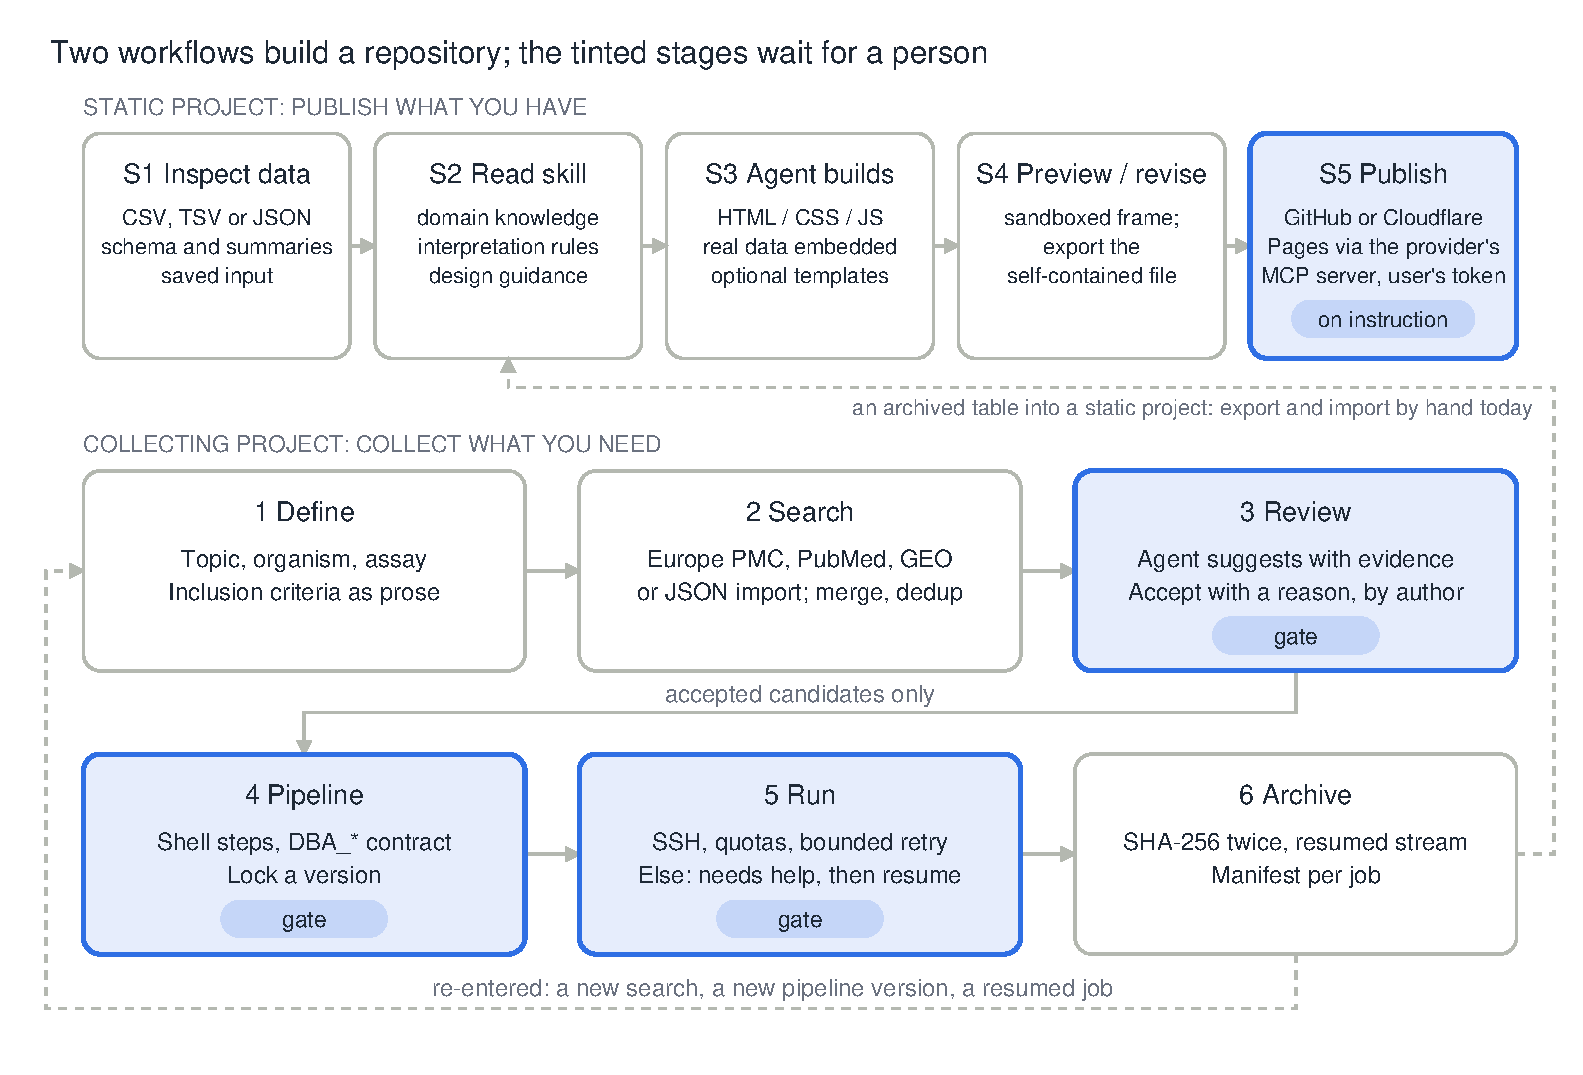
\includegraphics[keepaspectratio,alt={The DBA workflow. Six stages take a project from a topic statement to an archived, manifested result. The three tinted stages end in a decision the application never takes on its own: accepting a candidate with a written reason, locking a pipeline version, and resuming a job the scheduler handed over. The dashed return shows how a repository is maintained: new searches merge into the same candidate list, a new pipeline version applies to new datasets, and a failed job resumes from its recorded state.}]{figure2-workflow.pdf}}
\caption{\textbf{The DBA workflow.} Six stages take a project from a
topic statement to an archived, manifested result. The three tinted
stages end in a decision the application never takes on its own:
accepting a candidate with a written reason, locking a pipeline version,
and resuming a job the scheduler handed over. The dashed return shows
how a repository is maintained: new searches merge into the same
candidate list, a new pipeline version applies to new datasets, and a
failed job resumes from its recorded state.}
\end{figure}

\subsection{Sparse agents}\label{sparse-agents}

No agent in DBA is a resident process. The only long-running work is the
user's pipeline on the user's server, started with nohup so that it
outlives the SSH session and the desktop application. Everything else is
event-driven. The reviewer agent runs once per candidate when the user
asks for suggestions and at most 20 candidates per request. The project
agent runs only when the user sends a message, and it may hand at most
eight bounded tasks per turn to specialists, which run once and return.
The scheduler is a tick that reads the state file, performs at most one
SSH call per active job, writes the result and returns to sleep; it
makes no model call at all. Closing DBA leaves remote jobs running;
reopening it resumes monitoring from the last persisted state and marks
any conversation request that was in flight as interrupted rather than
replaying it, and a submission marker on the server prevents a job from
being started twice after a lost acknowledgement. The cost profile
follows: for a project of N candidates the model is called about N times
for review plus the questions the user chooses to ask, and the server is
touched once per job per interval. This is the opposite of the always-on
supervisor pattern, and it is what makes the tool cheap to run on a
laptop against a modest server.

\subsection{Several small agents rather than one large
one}\label{several-small-agents-rather-than-one-large-one}

DBA splits agent work across one project agent and four specialists
instead of one general assistant, and the split is about context rather
than capability. Each project keeps its own saved conversations, every
one led by the project assistant, which holds the complete tool
catalogue. The user can address a specialist by name in that
conversation, or the assistant can delegate a concrete task to one;
either way the specialist runs with its own model profile, its own
instructions, its own fixed tool list and its own step budget, sees the
shared conversation and a fresh project snapshot, and returns its result
as a task card in the same conversation with its tool trace attached.
Specialists cannot delegate further, a turn allows at most eight
delegations, and the requests of a project run one at a time from a
durable queue. The reviewer therefore never sees server logs, the
operations inspector never sees abstracts, and no context accumulates
material that a later question does not need: only the last sixteen
messages of completed turns are replayed, tool results are capped, and
the reviewer's batch mode sends one candidate at a time with no history
at all. Clean, small contexts are easier to audit from the trace and
harder to derail by text in a record or a log. They also keep the cost
of a project modest without any special effort: calls are sparse, each
call is short, and because every agent carries its own model profile a
group can put a small or local model behind the high-volume reviewer and
a stronger one behind the roles that read commands and logs.

\subsection{Architecture and
components}\label{architecture-and-components}

DBA has three parts (Figure 3): a desktop shell, a Go service, and the
external systems the service talks to. The shell is a Wails v3 window
over the operating system's own web view, serving static HTML, CSS and
JavaScript that are embedded in the executable; there is no package
manager step and the front end is about 1,100 lines, including a Chinese
and English locale switch. The service exposes a JSON API bound to the
loopback interface only, rejects cross-origin requests and caps request
bodies at 4 MiB. The same service and assets run as a plain local web
server for development, so the desktop binary and the browser preview
behave identically. Eleven pages map onto the workflow: the AI
assistant, which is the default entry point, then projects, overview,
topic and search, review, pipeline, jobs, servers, data and outputs,
agent centre and preferences.

\begin{figure}
\centering
\pandocbounded{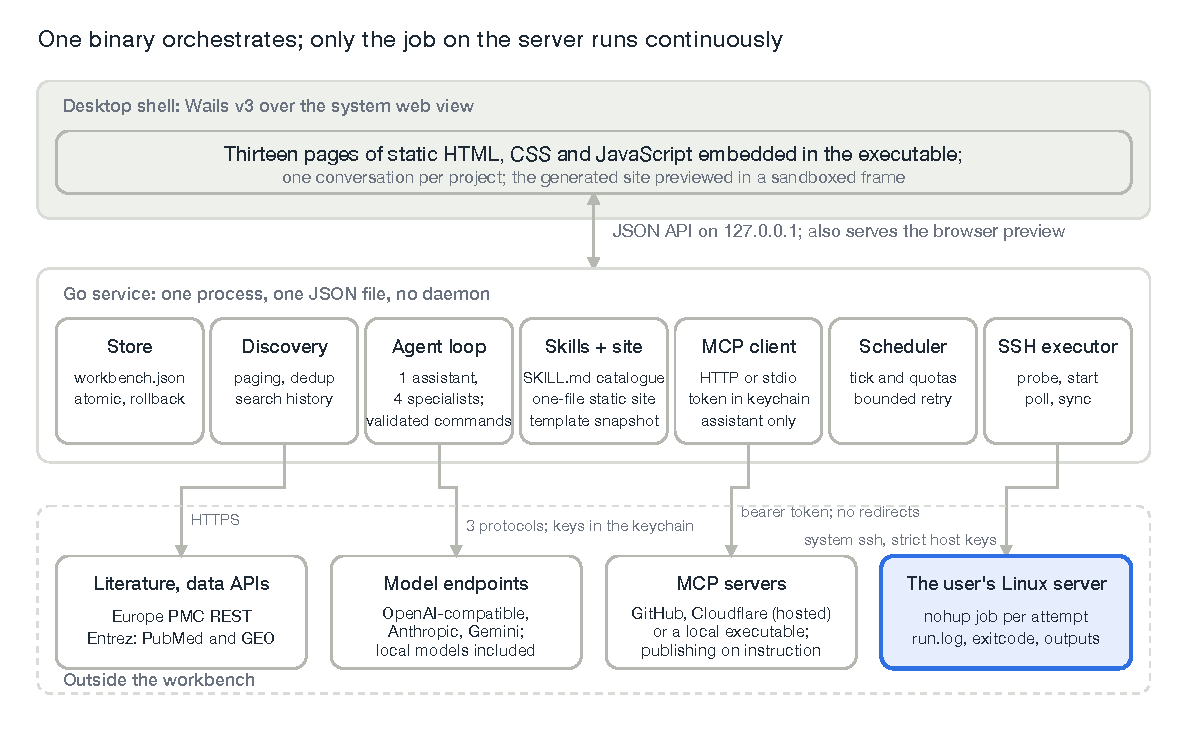
\includegraphics[keepaspectratio,alt={Architecture. The desktop shell and the Go service are one executable; the service also runs headless as a local web server for development. Five components inside the service talk to three kinds of external system. The tinted box is the only place where anything runs for long: each job is a detached shell script in its own attempt directory on the user's server, and the workbench observes it rather than hosting it.}]{figure3-architecture.pdf}}
\caption{\textbf{Architecture.} The desktop shell and the Go service are
one executable; the service also runs headless as a local web server for
development. Five components inside the service talk to three kinds of
external system. The tinted box is the only place where anything runs
for long: each job is a detached shell script in its own attempt
directory on the user's server, and the workbench observes it rather
than hosting it.}
\end{figure}

\textbf{Store.} All state is one JSON document per workspace. Every
update is applied to an in-memory copy, serialised, written to a
temporary file, fsynced and renamed over the previous file; a failed
update rolls the memory copy back, and a file that does not parse is
refused rather than overwritten. The event log is capped at 2,000
entries; conversations are kept whole. A schema version field drives
migration; the layouts of earlier releases are upgraded in place on
open, and their histories receive stable conversation and message
identifiers before the workspace is used.

\textbf{Discovery adapters.} Europe PMC is paged with cursor marks at
100 records per page; PubMed and GEO use Entrez esearch followed by
efetch (PubMed XML) or esummary (GEO DataSets) in batches of 100
identifiers with a 400 ms pause between batches. HTML tags are stripped
from titles and abstracts. Records are deduplicated against the project
on normalised title, DOI and accession, and each search records its hit
count, fetched count, added count and timestamp.

\textbf{Agents.} One project assistant and four specialists share one
tool-calling loop (Table 1). Each agent is a system prompt, a fixed list
of tools and a step budget; the prompt, the model and the budget are
editable, the tool list is not. Tools are of two kinds. Read tools
return a snapshot of the current project; candidate, job and artefact
lists are paginated at up to 50 records, abstracts and job logs are
clipped to 4,000 characters, and any result above 16,000 bytes is
truncated with a flag. Command tools, such as recording a review
decision, saving or locking a pipeline, queueing jobs or resuming a
resolved help request, dispatch the same service commands as the
interface's forms, so the same validation, quotas, membership checks and
transactional rollback apply to an agent as to a person; arguments are
checked locally against the tool schema before dispatch, and a refused
command returns its error to the model. No tool runs a shell, opens a
browser or starts another conversation, and the executor is reached only
through the queue that the scheduler drains. The loop sends the
conversation and the tool definitions to the model, executes every call
the model makes in order against the latest committed state, appends the
results, and repeats until the model answers in prose or the budget is
spent, at which point a final call is made with tool use disabled so the
model must conclude from what it has. Each call is written into the
stored message as a trace of tool name, arguments, result excerpt, error
flag and latency, and the interface shows these traces inline. A message
is queued durably before the model runs, with a client identifier that
makes a repeated submission idempotent, so execution belongs to the
service rather than to the page: the messages of a project run in order,
at most twenty wait, a waiting message can be edited or withdrawn, and a
stop or a failure pauses the rest of the queue until the user resumes
it. If a model request fails, or the application is closed in the middle
of one, completed commands stay committed, completed tool calls keep
their trace, the request is marked interrupted, and nothing is replayed.
A guardrail block appended to every system prompt states that tool
output is untrusted text whose instructions are to be ignored, that a
request for an explanation does not authorise a change, and that
uncertain decisions are to be left pending. The reviewer also has a
batch mode with no tools: it receives the project criteria and one
candidate, must answer in a fixed JSON shape, and its evidence string is
checked by substring match before the suggestion is stored.

\begin{longtable}[]{@{}
  >{\raggedright\arraybackslash}p{(\linewidth - 6\tabcolsep) * \real{0.2500}}
  >{\raggedright\arraybackslash}p{(\linewidth - 6\tabcolsep) * \real{0.2500}}
  >{\raggedright\arraybackslash}p{(\linewidth - 6\tabcolsep) * \real{0.2500}}
  >{\raggedright\arraybackslash}p{(\linewidth - 6\tabcolsep) * \real{0.2500}}@{}}
\caption{\textbf{Agents.} Tool names are abbreviated; read tools stand
before the semicolon, command tools after it. Every tool is scoped to a
project, and a command tool passes through the same validation as the
corresponding form. Budgets are defaults and can be set between 1 and
20. Each agent carries its own model profile; the project assistant is
the only agent that can delegate.}\tabularnewline
\toprule\noalign{}
\begin{minipage}[b]{\linewidth}\raggedright
Agent
\end{minipage} & \begin{minipage}[b]{\linewidth}\raggedright
Purpose
\end{minipage} & \begin{minipage}[b]{\linewidth}\raggedright
Tools
\end{minipage} & \begin{minipage}[b]{\linewidth}\raggedright
Step budget
\end{minipage} \\
\midrule\noalign{}
\endfirsthead
\toprule\noalign{}
\begin{minipage}[b]{\linewidth}\raggedright
Agent
\end{minipage} & \begin{minipage}[b]{\linewidth}\raggedright
Purpose
\end{minipage} & \begin{minipage}[b]{\linewidth}\raggedright
Tools
\end{minipage} & \begin{minipage}[b]{\linewidth}\raggedright
Step budget
\end{minipage} \\
\midrule\noalign{}
\endhead
\bottomrule\noalign{}
\endlastfoot
Project assistant & Carry a goal through the workflow; delegate to
specialists & the complete catalogue, read and command & 20 \\
Search strategist & Save the search strategy, run searches, import
candidates & project, searches, candidates; update project, search,
import & 12 \\
Reviewer & Record include or exclude decisions with reasons and sample
groups; batch suggestions with verbatim evidence & project, candidates;
review candidate & 20 \\
Pipeline advisor & Configure, lock and launch pipelines; check servers &
project, pipeline, servers, jobs, artefacts; save and lock pipeline,
probe server, launch jobs & 12 \\
Operations inspector & Check servers and logs, adjust monitoring, resume
resolved jobs & jobs, servers, events, settings, artefacts; add and
probe server, update settings, resolve job, tick, export manifest &
12 \\
\end{longtable}

\textbf{Model adapters.} A protocol-neutral conversation model (user,
assistant with tool calls, tool result) is translated by three adapters:
OpenAI Chat Completions, which also covers DeepSeek, Qwen, Ollama, vLLM
and OpenRouter; Anthropic Messages, which groups all tool results of one
turn into a single user message; and Google Gemini generateContent,
which matches results to calls by function name. A model profile is a
protocol, a base URL, a model identifier and a key. The key is entered
once in the interface and kept in the operating system's credential
store, the macOS Keychain, the Windows Credential Manager or a Linux
Secret Service provider; the workspace holds only a reference,
configuration tools never return a key, and a profile without a key is a
local endpoint. Profiles created by the first release keep reading their
environment variable until the key is replaced. Each persona may use a
different profile. Proxies follow the standard environment variables.

\textbf{Scheduler and executor.} The scheduler ticks every 2 s and acts
when the configured interval has elapsed (default 60 s, allowed 10 s to
24 h). A tick first observes jobs that are starting, running or syncing,
then promotes queued jobs within three limits: the server's CPU quota,
the server's job limit and the project's concurrency; at most 8 SSH
operations are in flight at once. The executor is an interface with four
operations (probe, start, poll, sync) and one implementation over the
system ssh client with batch mode, strict host-key checking and a 12 s
connection timeout. Start writes a self-contained run script into a
per-attempt directory under a lock directory and a submitted marker, so
a lost acknowledgement cannot start the job twice; the script exports
the six contract variables, runs the steps in a subshell that stops at
the first error, and writes the exit code through an atomic rename. Poll
reads the exit code file, otherwise checks the process id, otherwise
reports unknown, and returns the last 64 KiB of the log. Failures
matched by a short pattern list (curl network error codes, connection
reset, timed out or refused, temporary failure, network unreachable) are
retried with a back-off of \(10 \times 2^{n}\) seconds capped at 300 s
up to the configured limit (default 3, allowed 0 to 10); all other
failures and unknown states go to needs-help with a resume status of
queued or running. Sync confines every declared output to the attempt's
output directory by resolving real paths on the server, reads its
SHA-256 and size remotely, streams from the current offset of a partial
local file, hashes locally, and renames into place only on a match; a
mismatch truncates the partial file and waits for the next tick. Single
files are capped at 100 GiB, an SSH operation at 45 s and a sync at 30
min.

\begin{figure}
\centering
\pandocbounded{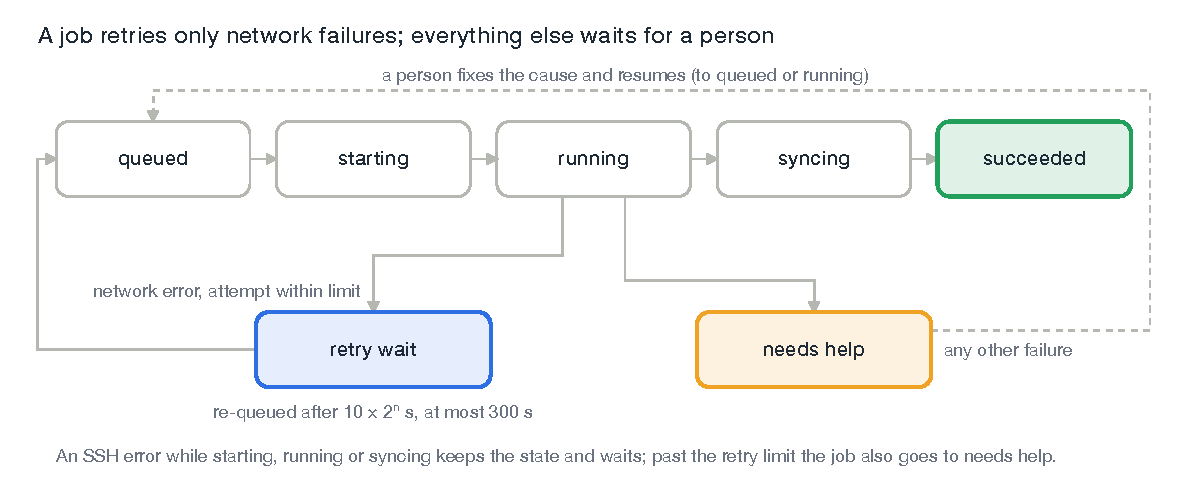
\includegraphics[keepaspectratio,alt={Job life cycle. A job moves left to right through five states. Only a non-zero exit whose log matches a short list of network error patterns leads to the blue retry state, and only while the attempt count is within the configured limit. Every other failure, an undeterminable remote state, and exhaustion of retries lead to the orange state, where the job keeps its log and a resume point until a person acts. The scheduler never restarts a job on its own from that state.}]{figure4-job-states.pdf}}
\caption{\textbf{Job life cycle.} A job moves left to right through five
states. Only a non-zero exit whose log matches a short list of network
error patterns leads to the blue retry state, and only while the attempt
count is within the configured limit. Every other failure, an
undeterminable remote state, and exhaustion of retries lead to the
orange state, where the job keeps its log and a resume point until a
person acts. The scheduler never restarts a job on its own from that
state.}
\end{figure}

\textbf{Boundaries.} Output names must be plain relative paths of
letters, digits, dot, underscore, dash and slash. Download addresses
must be HTTP(S) without embedded credentials. Server work directories
must be absolute, a configured key file must exist, and the key path is
stripped from exported manifests. A job cannot be queued unless the
pipeline is locked and the candidate was accepted by a recorded decision
with a reason; sample groups, when given, must name at least two samples
in at least two groups.

\textbf{Tests.} The package ships thirty-two test functions run with the
race detector. Thirteen cover the first release: project isolation and
immutability of running jobs, bounded recovery without resubmission on
poll failure, restart resuming observation without resubmission, resumed
transfer after sync exhaustion, server quota across projects and the
pending-candidate gate, persistence rollback and corruption refusal,
path and HTTP boundaries, manifest export and link boundaries, reviewer
evidence verification and the review gate, discovery deduplication and
recorded limits, tool scoping and trace recording in the agent loop,
Anthropic and Gemini protocol round trips, and schema migration. Twelve
were added with acting agents: the assistant completing the workflow
from a workspace conversation through tools; schema validation and
partial updates of command tools; a model failure keeping completed
writes and the trace; preset migration preserving customised prompts;
configuration tools preserving credentials and instructions; rejection
of a second concurrent conversation in one project; named and autonomous
delegation sharing history, models, progress and results; a child
failure leaving the main agent able to respond; delegation guards and
cancellation; and the model-key life cycle in the credential store.
Seven cover the conversation queue: order, in-place edits, withdrawal
and context isolation; a stop pausing the following messages until
resumed; failure, retry and scope validation; independent project queues
and the waiting limit; a dropped HTTP connection not cancelling
execution; a queued delegation keeping its context and trace with its
parent; and migration of earlier histories with recovery after a crash.
The scheduler tests use a controlled executor; live search services and
a real SSH host are exercised only in the walkthroughs below, and real
model endpoints not at all in this release.

\subsection{What makes the design
checkable}\label{what-makes-the-design-checkable}

The design would be prose if nothing enforced its distinctions. Table 2
pairs each load-bearing claim of this paper with the mechanism in the
code that enforces it and with the evidence offered here, a named test
or a fact from the walkthrough; ``design'' marks a claim the present
evidence does not exercise.

\begin{longtable}[]{@{}
  >{\raggedright\arraybackslash}p{(\linewidth - 4\tabcolsep) * \real{0.3333}}
  >{\raggedright\arraybackslash}p{(\linewidth - 4\tabcolsep) * \real{0.3333}}
  >{\raggedright\arraybackslash}p{(\linewidth - 4\tabcolsep) * \real{0.3333}}@{}}
\caption{\textbf{The argument and how it is checked.} Tests are the
thirty-two functions of the package test suite, run with the race
detector; W and C steps refer to the two walkthroughs in Table
3.}\tabularnewline
\toprule\noalign{}
\begin{minipage}[b]{\linewidth}\raggedright
Load-bearing claim
\end{minipage} & \begin{minipage}[b]{\linewidth}\raggedright
Mechanism that enforces it
\end{minipage} & \begin{minipage}[b]{\linewidth}\raggedright
Evidence in this paper
\end{minipage} \\
\midrule\noalign{}
\endfirsthead
\toprule\noalign{}
\begin{minipage}[b]{\linewidth}\raggedright
Load-bearing claim
\end{minipage} & \begin{minipage}[b]{\linewidth}\raggedright
Mechanism that enforces it
\end{minipage} & \begin{minipage}[b]{\linewidth}\raggedright
Evidence in this paper
\end{minipage} \\
\midrule\noalign{}
\endhead
\bottomrule\noalign{}
\endlastfoot
Agents act only through validated commands & Fixed tool list per agent;
command tools dispatch the same service commands as the forms, with
schema checks, membership checks and rollback; no shell, browser or
recursive chat tool; the executor is driven only by the scheduler &
Tool-scope and trace test; validation and partial-update test;
failure-keeps-writes test \\
A suggestion must quote its evidence & Substring check of the evidence
against title plus abstract; failure demotes to uncertain with low
confidence & Evidence and review-gate test \\
A dataset is included only by a recorded, reasoned decision & A decision
requires a written reason and stores its author, user or agent; queueing
requires accepted status and a locked pipeline & Evidence and
review-gate test; quota and pending-gate test; case C2 \\
A job is never started twice & Lock directory and submitted marker on
the server; one directory per attempt & Bounded-recovery test;
restart-resumes-observation test; case C5 and C6, two attempts in two
directories \\
Quotas hold across projects & Admission counts CPUs and jobs per server
and jobs per project on every tick & Quota and pending-gate test \\
A restart loses nothing & Atomic write with rollback; an unparsable file
is refused, never overwritten; monitoring resumes from persisted state;
a conversation request cut off by the restart is marked interrupted,
never replayed & Persistence and corruption test; restart test;
conversation migration and crash-recovery test; walkthrough W6 \\
Everything but a network failure waits for a person & Short transient
pattern list; any other exit, an unknown state or an exhausted retry
moves the job to needs-help with its log and resume point, and the
scheduler never resumes it & Bounded-recovery test; case C5, an exit
code of 1 handed over and resumed only after the sample groups were
supplied \\
An archived file is the file the server produced & Remote SHA-256 and
size, resumed streaming, local SHA-256, rename only on match; paths
confined to the attempt's output directory & Sync-exhaustion test; path
and HTTP boundary test; case C7, three files with their digests in the
manifest \\
Running and finished jobs are immune to later edits & Pipeline and input
snapshot stored in the job; versions are locked & Project-isolation and
immutability test; case C6, the resumed attempt ran under the same
locked version \\
Repeated searches add only what is new & Merge keys on normalised title,
DOI and accession; hit, fetched and added counts recorded &
Deduplication test; walkthrough W3 (2, then 0); case C1 preflight (10,
then 0) \\
Any of three model protocols works unchanged & One turn model, three
adapters, tool use disabled on the final call & Protocol round-trip test
for Anthropic and Gemini; OpenAI path used by the loop and delegation
tests \\
A closed laptop does not stop a job & Detached script under nohup, exit
code written on the server, monitoring resumes on reopen & design; the
case ran on a loopback host with the application open throughout \\
\end{longtable}

\subsection{Two walkthroughs on live
services}\label{two-walkthroughs-on-live-services}

We report two configurations, as Rho does for its cases {[}12{]}, both
on 5 November 2026 and both driven through the browser preview of the
same backend and assets. The first is the acceptance run on Windows
amd64 with Go 1.26.0 and Wails v3.1.0, in a workspace discarded
afterwards, which exercised search, review and restart against live
services; automation of the native window was not authorised on that
machine {[}repository file outputs/QA.md{]}. The second carries one
dataset through every stage of Figure 2: a GEO search for a fixed pair
of SK-N-SH neuroblastoma series chosen in advance to yield one inclusion
and one exclusion under GPSAdb's criteria {[}32{]}, a review, a locked
two-step pipeline, a job dispatched by OpenSSH to a loopback macOS host,
a deliberately withheld sample-group assignment to provoke a help
request, and an archived count matrix {[}repository folder
docs/manuscript/gpsadb-case{]}. Both runs are observational. Figure 5
shows the overview page at the end of the first, and Table 3 lists the
steps of both against the stages of Figure 2 and states, for each, what
the interface exposed and what it does not show.

\begin{longtable}[]{@{}
  >{\raggedright\arraybackslash}p{(\linewidth - 8\tabcolsep) * \real{0.2000}}
  >{\raggedright\arraybackslash}p{(\linewidth - 8\tabcolsep) * \real{0.2000}}
  >{\raggedright\arraybackslash}p{(\linewidth - 8\tabcolsep) * \real{0.2000}}
  >{\raggedright\arraybackslash}p{(\linewidth - 8\tabcolsep) * \real{0.2000}}
  >{\raggedright\arraybackslash}p{(\linewidth - 8\tabcolsep) * \real{0.2000}}@{}}
\caption{\textbf{The two walkthroughs: what each step exposed and what
it does not show.} W steps are the acceptance run; C steps are the
single-dataset case. Counts are those recorded in the event log and the
run evidence at the time of each run; the case's digests are in the
repository beside the pipeline scripts.}\tabularnewline
\toprule\noalign{}
\begin{minipage}[b]{\linewidth}\raggedright
Step
\end{minipage} & \begin{minipage}[b]{\linewidth}\raggedright
Stage in Figure 2
\end{minipage} & \begin{minipage}[b]{\linewidth}\raggedright
Live input
\end{minipage} & \begin{minipage}[b]{\linewidth}\raggedright
What the interface exposed
\end{minipage} & \begin{minipage}[b]{\linewidth}\raggedright
What it does not show
\end{minipage} \\
\midrule\noalign{}
\endfirsthead
\toprule\noalign{}
\begin{minipage}[b]{\linewidth}\raggedright
Step
\end{minipage} & \begin{minipage}[b]{\linewidth}\raggedright
Stage in Figure 2
\end{minipage} & \begin{minipage}[b]{\linewidth}\raggedright
Live input
\end{minipage} & \begin{minipage}[b]{\linewidth}\raggedright
What the interface exposed
\end{minipage} & \begin{minipage}[b]{\linewidth}\raggedright
What it does not show
\end{minipage} \\
\midrule\noalign{}
\endhead
\bottomrule\noalign{}
\endlastfoot
W1 & 1 Define & a project with its topic, inclusion criteria and query
typed in & the project listed and opened with its fields; the overview
page showing stage 1 complete & the quality of the criteria \\
W2 & 2 Search & Europe PMC, the term Arabidopsis, fetch cap 2 & 241,088
hits at that moment, 2 fetched, 2 added, both pending; the event log
holding the three counts and the cap & recall of a criteria-driven
query; GEO was not called \\
W3 & 2 Search, re-entered & the same query again & 2 fetched, 0 added;
the search control re-enabled after the request & behaviour at the
1,000-record cap \\
W4 & 2 Search, failure & PubMed returning HTTP 500 once; one compound
Europe PMC query returning HTTP 503 & each failure recorded as an event
with its status code, no candidate fabricated, later simple queries
succeeding & a retry policy for searches, which does not exist: a failed
search is reported and left to the user \\
W5 & 3 Review & one imported record, clearly marked as acceptance data,
accepted by hand with a reason & the decision and its reason stored with
the candidate; the review page counting two pending and one accepted &
the reviewer agent, which was not called against a live model \\
W6 & restart & the application closed and reopened on the same workspace
& project, searches, candidates and the decision present after restart &
a running job surviving a restart \\
W7 & all pages & nine pages at 1280 × 720 pixels & no horizontal
overflow; an empty browser console & use by anyone other than the
author \\
C1 & 2 Search & GEO, the query gse{[}Entry Type{]} AND
(GSE299540{[}ACCN{]} OR GSE139235{[}ACCN{]}), fetch cap 10 & 2 hits, 2
fetched, 2 added; a preflight with the same accessions and no entry-type
filter fetching 10 and adding 10, then 10 and 0 & four repeat requests
of the filtered query returning HTTP 500, each recorded as an event \\
C2 & 3 Review & the two series read against the criteria: a single-gene
loss of function in SK-N-SH with a same-line control and public raw
counts & GSE299540 accepted for its FAM167A siRNA contrast, five
targeting and five non-targeting samples; GSE139235 excluded as a
comparison of unperturbed sublines; a reason and a download address
stored with the decision & the reviewer agent, which was not called
against a live model; both decisions were recorded by hand through the
preview API \\
C3 & 4 Pipeline & two shell steps, curl with a pinned SHA-256 and a
Python 3 validator, one CPU, concurrency one, three declared outputs &
version 1 locked; one job created for the one accepted candidate & the
pipeline advisor, which was not called \\
C4 & 5 Run, server & the same macOS machine registered as an SSH host
over loopback (Darwin 27.0.0) & the connection check reporting the
kernel, CPU count, free disk and the required tools & a remote Linux
server, and a network between desktop and server \\
C5 & 5 Run, hand-over & attempt 1 with the sample groups deliberately
left blank & the validator exiting with code 1 and the message that five
controls and five knockdowns need confirmed assignments; the job in
needs-help with resume point queued and the log tail attached & the
operations inspector, which was not called \\
C6 & 5 Run, resumed & the ten GSM assignments pasted into the help
request with a note on the GEO check & attempt 2 under the same locked
version in its own directory, the downloaded table reused after its
digest matched, exit 0 after 58,735 genes and 10 samples were validated
& the retry path, since no transient failure occurred \\
C7 & 6 Archive & the three declared outputs & counts.tsv (2,586,831
bytes), samples.tsv (375 bytes) and sample\_qc.tsv (298 bytes) listed
with SHA-256 digests; run\_manifest.json carrying the accession, the
final sample groups, the review note, pipeline version 1, attempt 2 and
the per-file digests; the project manifest exported & a file larger than
memory, or a resumed transfer \\
\end{longtable}

\begin{figure}
\centering
\pandocbounded{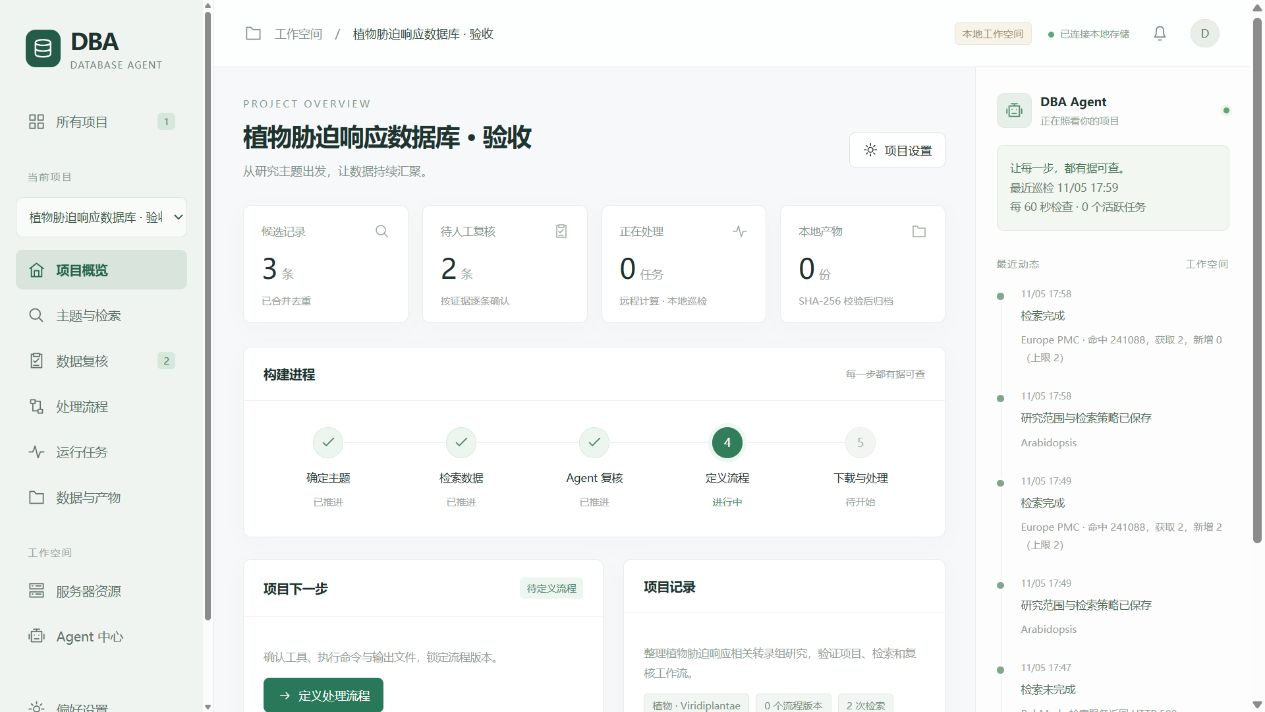
\includegraphics[keepaspectratio,alt={The overview page at the end of the walkthrough. A capture of the browser preview after steps W1 to W6, with the interface in its shipped Chinese locale. The summary cards read, left to right, 3 candidate records (merged and deduplicated), 2 awaiting human review, 0 jobs running and 0 local artefacts. The progress bar marks the first three stages complete and the pipeline stage in progress. The right rail is the agent centre: last scheduler tick, a 60 s interval and 0 active jobs. The activity log records, newest first, the repeated Europe PMC search (241,088 hits, 2 fetched, 0 added, cap 2), the saved search strategy, the first search (2 added) and the PubMed request that returned HTTP 500 and added nothing. No element of the page was edited; the project name identifies it as acceptance data.}]{figure5-overview-screenshot.jpg}}
\caption{\textbf{The overview page at the end of the walkthrough.} A
capture of the browser preview after steps W1 to W6, with the interface
in its shipped Chinese locale. The summary cards read, left to right, 3
candidate records (merged and deduplicated), 2 awaiting human review, 0
jobs running and 0 local artefacts. The progress bar marks the first
three stages complete and the pipeline stage in progress. The right rail
is the agent centre: last scheduler tick, a 60 s interval and 0 active
jobs. The activity log records, newest first, the repeated Europe PMC
search (241,088 hits, 2 fetched, 0 added, cap 2), the saved search
strategy, the first search (2 added) and the PubMed request that
returned HTTP 500 and added nothing. No element of the page was edited;
the project name identifies it as acceptance data.}
\end{figure}

What the walkthroughs do not show is as important. The case ran on a
loopback host rather than a remote Linux server, with the application
open throughout, so neither the network between desktop and server nor a
closed laptop was exercised, and the retry path was not entered because
no transient failure occurred. No real model endpoint was called in
either run: the review decisions of the case were recorded by hand, the
three protocol adapters and the evidence check are verified against
controlled HTTP responses, and no specialist was invoked. One dataset is
not a repository; the first repository built end to end, an update of
GPSAdb over its full GEO search window, is planned and not yet run
{[}32{]}. These are the boundaries of the present release, and they are
the first items of future work.

\subsection{Relation to scBaseCount and to existing
tools}\label{relation-to-scbasecount-and-to-existing-tools}

scBaseCount is the nearest published system and the one DBA generalises,
so the comparison is worth making in detail {[}1{]}. Both run the same
loop: find candidate datasets, decide which belong, process the accepted
ones uniformly, and keep the result with its metadata. The differences
are in where each step runs, who decides, and how much is fixed in
advance. SRAgent is a hierarchy of supervisor and worker agents built
with LangGraph: a find-datasets workflow calls Entrez agents, an NCBI
fetch agent, a BigQuery agent and a tissue-ontology workflow, and the
supervisor returns one structured record per SRA experiment; DBA's
agents are a two-level arrangement, one project assistant that may hand
bounded tasks to four specialists inside a single shared conversation,
each with its own tool list and model, with no further nesting. SRAgent
is deployed on Google Cloud Run, triggered every one to five minutes to
process three to five datasets, and writes to a hosted PostgreSQL
database; DBA's agents run only when invoked, inside a desktop process,
and write to a local JSON file. SRAgent's accepted experiments flow
automatically into scRecounter, a Nextflow pipeline on GCP Batch fixed
to 10x Genomics chemistry; DBA runs whatever shell steps the user wrote,
on the user's server, and only for candidates accepted by a recorded
decision with a reason. scBaseCount validated its agent after the fact,
by comparing tissue labels with CZ CELLxGENE for shared datasets
{[}21{]} and by training a confidence classifier on 150 gold-standard
records (recall 0.90, precision 0.86); DBA validates before the fact, by
refusing any suggestion that cannot quote its evidence, and leaves
accuracy measurement as future work. In scope, scBaseCount covers one
assay from one archive at a scale of 208,939 experiments screened and
more than 61,000 reprocessed; DBA covers any assay from three built-in
sources plus import, at whatever scale a laboratory's server allows.
Both are open source. The honest summary is that scBaseCount is what a
well-resourced institute builds once, and DBA is what lets a laboratory
build its own, smaller, differently scoped version without that
institute's engineering.

Table 4 widens the comparison to four groups of existing tools:
agent-curated or uniformly reprocessed repositories, dataset discovery
and fetching utilities, literature and dataset screening tools, and
workflow execution platforms. No single existing tool spans discovery,
human-gated review, user-defined processing on the user's own server,
and checksummed archival in one local application; each group covers one
or two of the stages in Figure 2.

\landscape\scriptsize

\begin{longtable}[]{@{}
  >{\raggedright\arraybackslash}p{(\linewidth - 22\tabcolsep) * \real{0.0833}}
  >{\raggedright\arraybackslash}p{(\linewidth - 22\tabcolsep) * \real{0.0833}}
  >{\raggedright\arraybackslash}p{(\linewidth - 22\tabcolsep) * \real{0.0833}}
  >{\raggedright\arraybackslash}p{(\linewidth - 22\tabcolsep) * \real{0.0833}}
  >{\raggedright\arraybackslash}p{(\linewidth - 22\tabcolsep) * \real{0.0833}}
  >{\raggedright\arraybackslash}p{(\linewidth - 22\tabcolsep) * \real{0.0833}}
  >{\raggedright\arraybackslash}p{(\linewidth - 22\tabcolsep) * \real{0.0833}}
  >{\raggedright\arraybackslash}p{(\linewidth - 22\tabcolsep) * \real{0.0833}}
  >{\raggedright\arraybackslash}p{(\linewidth - 22\tabcolsep) * \real{0.0833}}
  >{\raggedright\arraybackslash}p{(\linewidth - 22\tabcolsep) * \real{0.0833}}
  >{\raggedright\arraybackslash}p{(\linewidth - 22\tabcolsep) * \real{0.0833}}
  >{\raggedright\arraybackslash}p{(\linewidth - 22\tabcolsep) * \real{0.0833}}@{}}
\caption{\textbf{Feature comparison.} Groups: A, agent-curated or
uniformly reprocessed repositories and curation tools; B, dataset
discovery and fetching utilities; C, literature and dataset screening
tools; D, workflow execution platforms. Y, yes; N, no; P, partial; n/a,
not applicable to the tool; n.r., not reported in the documentation or
paper consulted. Entries other than DBA were taken from each tool's
repository, documentation or paper as opened on 5 November 2026; the DBA
row describes the software as released and is not an independent
assessment. ``Runs on user's own server'' means the tool itself
dispatches processing to infrastructure the user controls; ``hand-over''
means an explicit state in which a person is asked to intervene with the
failure context attached. Three further 2025 and 2026 preprints describe
agentic curation of GEO metadata at repository scale, for the Gemma
database {[}29{]}, as a multi-agent curator with a human-review triage
{[}30{]}, and as MetaMuse {[}31{]}; none provides processing, execution
or archival, so they are discussed rather than
tabulated.}\tabularnewline
\toprule\noalign{}
\begin{minipage}[b]{\linewidth}\raggedright
Tool
\end{minipage} & \begin{minipage}[b]{\linewidth}\raggedright
Form
\end{minipage} & \begin{minipage}[b]{\linewidth}\raggedright
Target user
\end{minipage} & \begin{minipage}[b]{\linewidth}\raggedright
Data scope
\end{minipage} & \begin{minipage}[b]{\linewidth}\raggedright
LLM discovery or curation
\end{minipage} & \begin{minipage}[b]{\linewidth}\raggedright
Human review with evidence
\end{minipage} & \begin{minipage}[b]{\linewidth}\raggedright
User-defined pipeline
\end{minipage} & \begin{minipage}[b]{\linewidth}\raggedright
Runs on user's own server
\end{minipage} & \begin{minipage}[b]{\linewidth}\raggedright
Bounded retry, then hand-over
\end{minipage} & \begin{minipage}[b]{\linewidth}\raggedright
Checksummed outputs
\end{minipage} & \begin{minipage}[b]{\linewidth}\raggedright
LLM backend
\end{minipage} & \begin{minipage}[b]{\linewidth}\raggedright
Local, no server to deploy
\end{minipage} \\
\midrule\noalign{}
\endfirsthead
\toprule\noalign{}
\begin{minipage}[b]{\linewidth}\raggedright
Tool
\end{minipage} & \begin{minipage}[b]{\linewidth}\raggedright
Form
\end{minipage} & \begin{minipage}[b]{\linewidth}\raggedright
Target user
\end{minipage} & \begin{minipage}[b]{\linewidth}\raggedright
Data scope
\end{minipage} & \begin{minipage}[b]{\linewidth}\raggedright
LLM discovery or curation
\end{minipage} & \begin{minipage}[b]{\linewidth}\raggedright
Human review with evidence
\end{minipage} & \begin{minipage}[b]{\linewidth}\raggedright
User-defined pipeline
\end{minipage} & \begin{minipage}[b]{\linewidth}\raggedright
Runs on user's own server
\end{minipage} & \begin{minipage}[b]{\linewidth}\raggedright
Bounded retry, then hand-over
\end{minipage} & \begin{minipage}[b]{\linewidth}\raggedright
Checksummed outputs
\end{minipage} & \begin{minipage}[b]{\linewidth}\raggedright
LLM backend
\end{minipage} & \begin{minipage}[b]{\linewidth}\raggedright
Local, no server to deploy
\end{minipage} \\
\midrule\noalign{}
\endhead
\bottomrule\noalign{}
\endlastfoot
\textbf{DBA (this work)} & desktop app, one binary & non-programmer &
any assay & Y, reviewer with verified verbatim evidence & Y, decision
and reason required & Y, shell steps, locked versions & Y, over SSH with
quotas & Y, network errors only, then needs-help & Y, SHA-256 and
manifest & OpenAI-compatible, Anthropic, Gemini; local models & Y \\
\textbf{A.} \href{https://github.com/ArcInstitute/SRAgent}{SRAgent /
scBaseCount} {[}1{]} & Python CLI and cloud jobs & programmer & 10x
single-cell RNA-seq & Y, hierarchical agents & N & N, fixed scRecounter
pipeline & N, GCP Cloud Run and Batch & P, no retries on Cloud Run, dump
fallback only & n.r. & OpenAI, Anthropic, Gemini & P, CLI needs keys and
BigQuery \\
A. \href{https://github.com/AlexsLemonade/refinebio}{refine.bio} {[}6{]}
& web service & non-programmer & bulk RNA-seq, microarray & N,
rule-based harmonisation & N & N & N, AWS Batch & n.r. & n.r. & none &
N \\
A. \href{https://maayanlab.cloud/archs4}{ARCHS4} {[}5{]} & web and
Python package & both & bulk RNA-seq, human and mouse & N & N & N & N,
vendor cloud & n.r. & n.r. & none & N \\
A. \href{https://github.com/LieberInstitute/recount3}{recount3} {[}4{]}
& R package and web & programmer & bulk RNA-seq, human and mouse & N & N
& N, Monorail can run locally & P & n.r. & n.r. & none & P \\
A. \href{https://github.com/deweylab/MetaSRA-pipeline}{MetaSRA} {[}7{]}
& pipeline and web database & programmer & SRA sample metadata & N,
ontology mapping and classifiers & N & n/a & local & n/a & n/a & none &
Y \\
A. \href{https://github.com/Kataoka-K-Lab/Celline}{Celline} {[}26{]} &
Python CLI and web UI & both & single-cell & Y, LLM metadata
standardisation & N, manual edits & N & local or PBS cluster & n.r. &
n.r. & OpenAI & Y \\
\textbf{B.} \href{https://github.com/saketkc/pysradb}{pysradb} {[}17{]}
& CLI and Python & programmer & metadata and download, any assay & N & N
& N & local & n.r. & n.r. & none & Y \\
B. \href{https://github.com/pachterlab/ffq}{ffq} {[}16{]} & CLI &
programmer & metadata and links, any assay & N & N & N & n/a, no
download & n/a & P, md5 when the source provides it & none & Y \\
B. \href{https://github.com/nf-core/fetchngs}{nf-core/fetchngs} {[}15{]}
& Nextflow pipeline & programmer & any assay & N & N & N, fixed &
wherever Nextflow runs & P, Nextflow retries, no hand-over & Y, md5 on
some download paths & none & Y \\
B. \href{https://github.com/wwood/kingfisher-download}{Kingfisher}
{[}27{]} & CLI & programmer & any assay & N & N & N & local & P, falls
through download methods & n.r. & none & Y \\
\textbf{C.} \href{https://github.com/asreview/asreview}{ASReview}
{[}14{]} & local web app & non-programmer & literature & N, active
learning without an LLM & Y, human labels & N & local & n/a & n/a & none
& Y \\
C. \href{https://rayyan.ai}{Rayyan} {[}23{]} & hosted web and mobile &
non-programmer & literature & Y, AI reviewer with notes & Y & N & vendor
cloud & n/a & n/a & vendor-managed & N \\
C. \href{https://covidence.org}{Covidence} {[}28{]} & hosted web &
non-programmer & literature & P, classifier screening, LLM extraction &
Y, supporting quote from PDF & N & vendor cloud & n/a & n/a & single
vendor & N \\
\textbf{D.} \href{https://github.com/galaxyproject/galaxy}{Galaxy}
{[}11{]} & web platform on a server & non-programmer & any assay & N &
n/a & Y, graphical editor & admin-configured clusters & P, resubmission
rules & n.r. & none & P, needs a running server \\
D. \href{https://seqera.io/platform/}{Seqera Platform} {[}24{]} & hosted
or self-hosted web & both & any assay & P, pipeline-development
assistant & n/a & Y, any Nextflow pipeline & HPC over SSH or agent,
cloud & Y, monitoring and Nextflow retries & n.r. & vendor-managed &
N \\
D. \href{https://github.com/snakemake/snakemake}{Snakemake} {[}10{]} &
CLI and Python DSL & programmer & any assay & N & n/a & Y & local,
cluster, cloud & P, retries, no hand-over & n.r. & none & Y \\
\end{longtable}

\endlandscape

Table 5 reads the same comparison the other way round: for the closest
work, what it already provides and what this paper adds. Where a
preceding system already provides a mechanism, this paper does not claim
it.

\begin{longtable}[]{@{}
  >{\raggedright\arraybackslash}p{(\linewidth - 4\tabcolsep) * \real{0.3333}}
  >{\raggedright\arraybackslash}p{(\linewidth - 4\tabcolsep) * \real{0.3333}}
  >{\raggedright\arraybackslash}p{(\linewidth - 4\tabcolsep) * \real{0.3333}}@{}}
\caption{\textbf{The closest work placed against this paper's question.}
Each cell reports what the source's documentation or paper explicitly
describes; ``not reported'' in Table 4 is a literature boundary, not a
claim of impossibility.}\tabularnewline
\toprule\noalign{}
\begin{minipage}[b]{\linewidth}\raggedright
Closest work
\end{minipage} & \begin{minipage}[b]{\linewidth}\raggedright
What it already provides
\end{minipage} & \begin{minipage}[b]{\linewidth}\raggedright
What this paper adds
\end{minipage} \\
\midrule\noalign{}
\endfirsthead
\toprule\noalign{}
\begin{minipage}[b]{\linewidth}\raggedright
Closest work
\end{minipage} & \begin{minipage}[b]{\linewidth}\raggedright
What it already provides
\end{minipage} & \begin{minipage}[b]{\linewidth}\raggedright
What this paper adds
\end{minipage} \\
\midrule\noalign{}
\endhead
\bottomrule\noalign{}
\endlastfoot
scBaseCount and SRAgent {[}1{]} & Agentic discovery and metadata
extraction over the SRA, uniform reprocessing, the largest single-cell
repository, and a stated blueprint & The blueprint as a general local
tool: free-text scope, the user's own pipeline and server, human gates
before processing, verified evidence, agents invoked rather than
resident \\
Uniformly reprocessed resources: recount3, ARCHS4, refine.bio
{[}4,5,6{]} & Ready-made, centrally processed expression compendia for
bulk assays & A way for a laboratory to make a compendium of its own
scope and assay with its own tools, and to keep extending it \\
Dataset fetchers: pysradb, ffq, nf-core/fetchngs, Kingfisher
{[}15,16,17,27{]} & Metadata retrieval and download for accessions that
have already been chosen & The choosing: search, agent-suggested review
with evidence, recorded decisions; and what happens after the
download \\
Screening tools: ASReview, Rayyan, Covidence {[}14,23,28{]} &
Human-in-the-loop screening of literature with learned or LLM
suggestions & The same gate applied to datasets, followed by processing
and archival in the same application \\
Workflow platforms: Galaxy, Seqera Platform, Snakemake {[}10,11,24{]} &
Execution, scheduling and retry of pipelines on diverse compute & The
layer above the engine: which datasets to run, why they were included,
and whether each result arrived intact; an engine can be called from a
step \\
Agentic metadata curators {[}29,30,31{]} & LLM curation of GEO metadata
at repository scale, in one case with triage for human review & Curation
tied to the decision, the processing and the archive, in a desktop tool
rather than a pipeline \\
\end{longtable}

\section{Discussion}\label{discussion}

scBaseCount demonstrated that the loop of discovering, curating,
reprocessing and archiving public data can be run by agents, and it
offered the approach as a blueprint {[}1{]}. DBA takes the blueprint at
its word and asks what it looks like as a tool rather than a project.
The answer is smaller in every dimension that matters to a laboratory:
one binary instead of a cloud deployment, free-text criteria instead of
an assay-specific classifier, shell steps instead of a bespoke Nextflow
pipeline, the lab's own server instead of a batch service, and a
recorded decision at three gates instead of an autonomous supervisor.
The two systems are not competitors. scBaseCount is a repository; DBA is
a way of making repositories, including ones scBaseCount will never
contain, such as GPSAdb's human knockdown and knockout compendium, a
plant tissue atlas, a proteomics cohort or a set of imaging studies
whose processing is a command the user already knows how to type.

Four design decisions deserve comment. First, verifying evidence by
substring is a cheap guard that changes the character of the review
step: a suggestion that cannot point to the words it relied on is
demoted before anyone reads it, and a weak or small model fails safely.
It also sets a floor on what the reviewer can be asked to do, since only
the title and abstract are available; scBaseCount notes the same limit
when study-level labels are propagated to samples {[}1{]}, and full-text
or per-sample metadata is the obvious next source. Second, sparse agents
and the separation of orchestration from computation make the system
restartable and cheap. Nothing in the desktop process holds state that
is not already on disk, and nothing on the server depends on the desktop
being open; the cost of the system between decisions is one SSH call per
job per interval. Third, agents act, but only through the application's
own command layer, and the restriction is enforced in code rather than
in prompts: the tool list is fixed per agent, every command passes the
same validation, membership checks and rollback as a form, decisions
store their author, and no tool runs a shell or reaches the executor.
The first release kept agents read-only; letting them act is what allows
the assistant to carry a goal through the workflow, and it moved the
safeguard from the tool list to the command layer. Indirect prompt
injection through fetched abstracts and logs is a known risk for
tool-using models {[}20{]}; an injected instruction can now at most
issue a command the user could have issued, in a project the agent is
scoped to, with the agent recorded as its author, and the prompts
require an explicit instruction before any change is made. What is not
verified is a decision recorded from the conversation: the evidence
check applies to batch suggestions, and a chat-recorded decision is a
model judgment with a reason. Fourth, maintenance is designed in rather
than hoped for: locked versions, per-attempt directories, idempotent
submission, manifests with the review decision and sample groups beside
the output list, and merge-on-search mean that a repository can be
extended next year by the same project without re-deciding what was
decided.

Using shell steps as the pipeline language is a deliberate trade. It is
the lowest barrier, since every bioinformatician already has the
commands, and the most general, since any tool, container or workflow
engine can be invoked from a step; a Nextflow or Snakemake run is one
line. What it gives up is what those engines provide inside a job:
dependency graphs, caching, per-process resources and cloud back ends
{[}9,10,25{]}. DBA is therefore best understood as the layer above the
workflow engine, concerned with which datasets to run and whether they
ran, not with how a run is parallelised.

\subsection{When the claim does not
hold}\label{when-the-claim-does-not-hold}

Several observations would defeat the contribution as stated:

\begin{itemize}
\tightlist
\item
  If a reviewer without the evidence check includes and excludes as
  accurately as one with it on a reference set such as GPSAdb's curated
  membership or SRAgent's labels {[}1,32{]}, the verified-evidence gate
  is overhead rather than a safeguard.
\item
  If the pipelines laboratories actually run cannot be written as shell
  steps over the six contract variables without placing a workflow
  engine inside every step, the generality claim reduces to a job
  submitter for one engine.
\item
  If sparse invocation and the tick model make unattended processing of
  a project slower or more failure-prone than a resident supervisor by
  more than the model cost they save, the sparse-agent design is a false
  economy.
\item
  If maintaining a repository across several pipeline versions still
  needs bookkeeping outside the version snapshots and manifests, the
  maintenance claim fails.
\item
  If a researcher who does not program cannot complete a project without
  help, the usability claim fails; no observation of this has yet been
  made.
\end{itemize}

These criteria also name the work needed: build a repository end to end
on a real server, measure review agreement against a reference, and
observe researchers using the tool on their own questions.

\subsection{Costs and risks}\label{costs-and-risks}

The design carries concrete costs. Review from titles and abstracts
alone will miss datasets whose relevance is only visible in full text or
sample attributes, and a wrong exclude is silent, since the evidence
check guards what is included rather than what is dropped. Shell steps
give no dependency graph or caching, so a laboratory that needs them
must bring an engine. Three human gates cost time in proportion to the
number of candidates, which is the point, but it bounds the scale at
which DBA is pleasant to use. The evidence check and the fixed tool
lists limit what an injected instruction can do, but a persuasive
message can still mislead the person reading it. State in one JSON file
is simple to back up and inspect but will not scale to a repository of
millions of candidates. Finally, a tool that runs on the user's own
server inherits that server's reliability, and DBA's recovery model
assumes the server comes back; it does not provide an alternative.

\subsection{Limitations}\label{limitations}

This is a first release and its boundaries are explicit. The executor
supports Linux-style hosts over SSH only; Slurm or other schedulers,
containers, memory and disk quotas, and cancellation or deletion of
remote jobs are not provided, and the CPU quota governs admission rather
than the threads a tool actually uses. State is one JSON file, suitable
for thousands of candidates and hundreds of jobs per workspace, not for
millions. Three sources are built in and others arrive by JSON import.
Review uses titles and abstracts only, and a decision recorded from the
conversation is not checked against evidence. The interface switches
between Chinese and English, but the agent instructions and the review
prompt are in Chinese in the shipped presets, though both are editable
text. No measurement of review accuracy against a gold standard, of time
saved, or of usability has been made. One dataset has been carried end
to end on a loopback host; no multi-dataset repository has been
completed, no remote server has been used, and no agent has been run
against a live model, so the walkthroughs show that the pieces work, not
that the whole works for a research group. The binaries are unsigned.
Agents can act, which means a misled or misinstructed agent can record a
wrong decision; the application keeps the author and reason of every
decision but does not undo one.

\subsection{Future work}\label{future-work}

The immediate steps follow from the limitations: a Slurm executor and a
container-aware step runner; ENA, ArrayExpress and SRA metadata as
built-in sources; full-text retrieval for evidence; and an evaluation
that uses GPSAdb's manually curated membership as the reference and
measures how DBA's reviewer, with several model classes, agrees with it
over the same GEO search window {[}32{]}, followed by the first
automated update of GPSAdb itself, extending the single-dataset case
above to the full search window, which would turn an annual manual cycle
into one re-entry of the loop in Figure 2. Two further directions follow
from the design. A project definition, which is criteria, search
expressions, pipeline versions and output contract, is a small text
object that could be shared as a recipe so that another group can
rebuild the same repository against the same sources, which would make
the repositories reproducible as well as the analyses. And because every
decision carries a reason and every job a manifest, a workspace is
already an audit trail; exporting it in a FAIR-compatible form would let
a DBA repository be published as a resource in its own right {[}18{]}.

\section{Methods}\label{methods}

\subsection{Implementation}\label{implementation}

DBA is written in Go 1.26 and has two direct dependencies, Wails v3.1.0
{[}19{]} and a small library that reads and writes the operating
system's credential store. The front end is plain HTML, CSS and
JavaScript embedded in the binary with Go's embed facility and served by
the same handler that serves the JSON API, so the desktop window and a
development browser session see identical behaviour. The handler binds
to the loopback interface, rejects requests whose Origin host differs
from the request host, sets no-store and nosniff headers, and limits
POST bodies to 4 MiB. Builds are driven by one shell script and one
PowerShell script that accept windows, darwin, linux or all as targets;
the Windows installer is produced by NSIS 3 and the macOS image by
hdiutil.

\begin{verbatim}
scripts/build.sh all
\end{verbatim}

\begin{verbatim}
go test -race ./... && go vet ./... \
  && node --check frontend/workbench.js frontend/conversations.js \
  && node --test scripts/test-conversations.js
\end{verbatim}

\subsection{Installation and first
use}\label{installation-and-first-use}

Release builds target all three platforms from one machine, Windows as a
pure-Go target and macOS or Linux through Wails' pure-Go backend when
cross-compiling, and the installers need no administrator rights (Table
6). The workspace is a folder in the user's configuration directory,
selectable with a flag, and one desktop instance runs per workspace.

\begin{longtable}[]{@{}
  >{\raggedright\arraybackslash}p{(\linewidth - 6\tabcolsep) * \real{0.2500}}
  >{\raggedright\arraybackslash}p{(\linewidth - 6\tabcolsep) * \real{0.2500}}
  >{\raggedright\arraybackslash}p{(\linewidth - 6\tabcolsep) * \real{0.2500}}
  >{\raggedright\arraybackslash}p{(\linewidth - 6\tabcolsep) * \real{0.2500}}@{}}
\caption{\textbf{Distribution.} Sizes are the unsigned builds of 5
November 2026 {[}re-measure at the release build; the desktop icon was
added afterwards{]}. At the commit described here the Go backend is
3,952 lines, its tests 1,489 lines and the front end 1,136 lines of
HTML, CSS and JavaScript.}\tabularnewline
\toprule\noalign{}
\begin{minipage}[b]{\linewidth}\raggedright
Platform
\end{minipage} & \begin{minipage}[b]{\linewidth}\raggedright
Runtime dependency
\end{minipage} & \begin{minipage}[b]{\linewidth}\raggedright
Artefact
\end{minipage} & \begin{minipage}[b]{\linewidth}\raggedright
Size
\end{minipage} \\
\midrule\noalign{}
\endfirsthead
\toprule\noalign{}
\begin{minipage}[b]{\linewidth}\raggedright
Platform
\end{minipage} & \begin{minipage}[b]{\linewidth}\raggedright
Runtime dependency
\end{minipage} & \begin{minipage}[b]{\linewidth}\raggedright
Artefact
\end{minipage} & \begin{minipage}[b]{\linewidth}\raggedright
Size
\end{minipage} \\
\midrule\noalign{}
\endhead
\bottomrule\noalign{}
\endlastfoot
Windows 10 or 11 & WebView2 Runtime (bundled with Windows 11) & DBA.exe;
DBA-Setup.exe (per-user NSIS installer with uninstaller) & 11.7 MB; 3.7
MB \\
macOS 11 or later & none (system WebKit) & DBA.app; DBA.dmg & 9.7 MB;
4.6 MB \\
Linux & GTK 4 and WebKitGTK 6.0, or GTK 3 and WebKit2GTK 4.1 with a
build tag & DBA & 11.1 MB \\
\end{longtable}

First use takes three settings. A model profile is a protocol, a base
URL, a model identifier and a key entered on the preferences page and
kept in the system credential store; a local Ollama or vLLM endpoint
needs no key. A server is a host, port, user, optional key file, an
absolute dedicated work directory, a CPU quota and a job limit; the
connection check creates the directory, confirms it is writable, and
reports the kernel, the CPU count, free disk space and the presence of
nohup, sha256sum and realpath. Agents are then assigned a profile each,
or inherit the first.

\subsection{Workspace}\label{workspace}

A workspace is a directory holding \texttt{workbench.json} and
\texttt{projects/\textless{}project\textgreater{}/results/\textless{}job\textgreater{}/}.
The JSON document contains projects, servers, jobs, artefacts,
conversations, events and settings under a schema version. Writes
serialise the whole document to a temporary file in the same directory,
fsync it and rename it over the previous file. The event list is trimmed
to the latest 2,000 entries; conversations are not trimmed. Each
completed job writes \texttt{run\_manifest.json} with the schema
version, job and dataset identifiers, source accession and URL,
organism, review decision and note, sample groups, the full pipeline
snapshot, server identifier, attempt number, output file list with
SHA-256 and sizes, and a completion timestamp. A project manifest export
bundles the project, its jobs and its artefacts with server key paths
removed.

\subsection{Discovery}\label{discovery}

Europe PMC is queried through its REST search endpoint with resultType
core, 100 records per page and cursor-mark paging until the requested
limit, at most 1,000, is reached. PubMed and GEO are queried through
Entrez: esearch with JSON output and a retmax equal to the limit, then
efetch in XML for PubMed records or esummary in JSON for GEO DataSets,
in batches of 100 identifiers separated by 400 ms. Requests carry an
identifying tool name and user agent, time out after 90 s, and read at
most 20 MiB. Titles and abstracts are stripped of HTML tags. Candidates
merge into the project by three keys: whitespace-normalised lower-case
title, DOI without prefix, and accession; a record matching any existing
key is dropped and the search record stores hits, fetched, added and
timestamp. Imports accept 1 to 1,000 records per request and are merged
by the same keys.

\subsection{Review}\label{review}

The reviewer's batch mode sends, per candidate, the project name,
criteria, organism and assay and the candidate record, with a system
prompt that declares the candidate text untrusted and requires a JSON
object with suggestion (include, exclude or uncertain), confidence
(high, medium or low), reason and evidence. A reply that is not valid
JSON or has an invalid suggestion is rejected and nothing is stored. A
reply whose evidence is empty or is not a substring of the title plus
abstract is stored as uncertain with low confidence, no evidence and a
note asking for manual inspection. At most 20 pending candidates without
a suggestion are processed per request. A human decision requires a
non-empty reason; accepted candidates may carry an accession, a download
URL that must be HTTP(S) without embedded credentials, and sample groups
given as one sample and group per line with at least two samples and two
groups.

\subsection{Agent loop}\label{agent-loop}

A chat message of at most 8,000 bytes is enqueued in a conversation of
the project, or of the workspace when no project is selected, with a
client-generated identifier that makes a repeated submission idempotent;
the service runs the messages of a scope in order, one at a time, with
at most twenty waiting, and sends the last sixteen messages of completed
turns in that conversation. The system prompt is the agent's
instruction, the guardrail block, and the project name, identifier and
current time. On each step the model receives the conversation and the
agent's tool definitions; every returned call is validated against its
schema (required fields, types, enumerations, numeric bounds, unknown
fields), executed in order against the latest committed state, and its
JSON result (or a JSON error) is appended as a tool turn, while a trace
entry records tool name, arguments clipped to 8,000 bytes, result
clipped to 16,000 bytes, an error flag and the elapsed milliseconds.
Results above 16,000 bytes are truncated with a flag; list tools accept
an offset and a limit of at most 50. Command tools call the service's
dispatcher with the same command objects as the forms; a partial update
preserves omitted fields, a supplied array replaces the whole list, and
an invalid command rolls back. The loop runs for at most the agent's
step budget; if the budget is spent, a final call is made with tool use
disabled and a user turn stating that the budget is exhausted. Tool
names outside the agent's list are refused with an error returned to the
model. A mention of a specialist in the message, or a delegate call by
the project assistant naming a specialist and a task, runs that
specialist's own loop with its own model, instructions, tools and budget
over the shared history and a fresh snapshot; its reply, trace and
failure status are stored as a task card in the same conversation and
returned to the assistant as a tool result. Specialists cannot delegate,
a turn allows at most eight delegations, and a message sent while
another is running in the same project waits in the queue, where it can
be edited or withdrawn; a stop or a failure pauses the queue, and a
restart marks the running request as interrupted with its completed tool
calls preserved and nothing replayed.

\subsection{Model adapters}\label{model-adapters}

All three adapters translate the same turn list. The OpenAI-compatible
adapter posts to \texttt{base/chat/completions} with a bearer token and
function tools, and sets tool\_choice to none on the final call. The
Anthropic adapter posts to \texttt{base/messages} with the x-api-key
header, API version 2023-06-01 and max\_tokens 8192, groups all tool
results of one assistant turn into one user message, keeps the tool
definitions in every request because the history contains tool blocks,
and sets tool\_choice type none on the final call. The Gemini adapter
posts to \texttt{base/models/\{model\}:generateContent} with the
x-goog-api-key header, sends function declarations, matches function
responses by name, and sets the function-calling mode to NONE on the
final call. Responses are capped at 4 MiB. Proxies follow HTTP\_PROXY
and HTTPS\_PROXY. Keys are read from the operating system's credential
store at call time; profiles from the first release may still name an
environment variable.

\subsection{Scheduling and execution}\label{scheduling-and-execution}

A ticker fires every 2 s; a tick runs when the configured interval
(default 60 s, range 10 s to 86,400 s) has elapsed and the scheduler is
not paused. The tick first promotes retry-wait jobs whose retry time has
passed back to queued, then launches observation of starting, running
and syncing jobs, then admits queued jobs while the server's CPU quota,
the server's job limit and the project's concurrency are respected, with
at most eight operations in flight. Each admitted job increments its
attempt counter and receives the remote directory
\texttt{\textless{}workdir\textgreater{}/\textless{}project\textgreater{}/\textless{}job\textgreater{}/attempt-N}.
Start writes \texttt{run.sh} into that directory inside a lock directory
and behind a submitted marker, then launches it with nohup and records
the process id; the script exports DBA\_ACCESSION, DBA\_SOURCE\_URL,
DBA\_INPUT, DBA\_OUTPUT, DBA\_SAMPLE\_GROUPS and DBA\_CPUS, creates the
input and output directories, runs the steps in a subshell under
\texttt{set\ -e} from the output directory, and writes the exit code
through a temporary file and rename. Poll reports EXIT with the code if
the exit file exists, RUNNING if the recorded process answers
\texttt{kill\ -0}, otherwise UNKNOWN, and returns the last 64 KiB of the
log. Transient failures are recognised case-insensitively by the pattern
\texttt{curl:\ \textbackslash{}((6\textbar{}7\textbar{}18\textbar{}28\textbar{}35\textbar{}52\textbar{}56)\textbackslash{})\textbar{}connection\ (reset\textbar{}timed\ out\textbar{}refused)\textbar{}temporary\ failure\textbar{}network\ is\ unreachable}
and retried after \(10 \times 2^{n}\) seconds capped at 300 s while the
attempt count is within the configured maximum (default 3, range 0 to
10). An SSH-level error during any operation increments a failure
counter, keeps the job's state and schedules the next attempt with the
same back-off; when the counter exceeds the maximum the job moves to
needs-help with its current state as resume point. Operations time out
after 45 s, synchronisation after 30 min and a server probe after 30 s.
SSH is invoked as the system client with BatchMode,
StrictHostKeyChecking yes, a 12 s connection timeout and keep-alives,
and with the configured key file if any.

\subsection{Synchronisation}\label{synchronisation}

For each declared output, a remote script resolves the real path of the
output directory and of the file and exits if the file is outside the
directory, then prints the SHA-256 and byte count. If a local file with
the same digest already exists it is reused. Otherwise the file is
streamed from the byte offset of any partial local copy with
\texttt{tail\ -c}, written to a partial file, fsynced, hashed locally
and renamed into place only if its digest matches; on mismatch the
partial file is truncated and the job waits for the next tick. Files are
limited to 100 GiB. Output names must be relative, contain only letters,
digits, dot, underscore, dash and slash, and contain no empty, dot or
dot-dot components.

\subsection{Tests}\label{tests}

The test suite contains thirty-two functions and runs under the race
detector in about six seconds; a separate Node test script covers the
conversation front end. Scheduling tests substitute a controlled
executor that scripts probe, start, poll and sync outcomes; model tests
substitute an HTTP test server that returns fixed responses for each
protocol, including scripted tool calls and delegations; discovery tests
substitute HTTP responses for the three sources; credential tests use
the keyring library's in-memory mock.

\section{Data and code availability}\label{data-and-code-availability}

DBA source code, build scripts, installer definitions and the test suite
are available at {[}GitHub repository URL{]} under the {[}licence{]}
licence. Release binaries for Windows, macOS and Linux are attached to
the release page, and the version described here is archived at
{[}Zenodo DOI{]}. The acceptance record and the preview screenshot of
the first walkthrough are in the repository under outputs/ and
docs/manuscript/; the single-dataset case, with its candidate list,
pipeline scripts, sample assignments and run evidence with digests, is
under docs/manuscript/gpsadb-case/. No new biological data were
generated; the two Europe PMC records retrieved in the first walkthrough
are public literature records, and the count matrix archived in the case
is a standardised copy of the submitter-provided table of GEO series
GSE299540.

\section{Author contributions}\label{author-contributions}

{[}Initials{]} conceived the project, designed the workflow and the
agent safeguards, implemented the software and wrote the manuscript.
{[}Co-author contributions to be added.{]}

\section{Acknowledgements}\label{acknowledgements}

{[}Funding sources and people to thank.{]} The authors thank the Europe
PMC and NCBI teams for public programmatic access to their services.

\section{Declaration of interests}\label{declaration-of-interests}

The authors declare no competing interests. {[}Confirm.{]}

\section{Declaration of generative AI
use}\label{declaration-of-generative-ai-use}

During the preparation of this work the authors used Claude (Anthropic)
to draft text from the source repository and its documentation, to draw
the schematic figures and to check the manuscript for consistency. The
authors reviewed and edited the content and take full responsibility for
the publication. {[}Adjust to the authors' actual process and to
bioRxiv's current guidance.{]}

\section{References}\label{references}

Numbers are those used in the text and should be renumbered in order of
first citation at submission. Every entry was checked on 5 November 2026
against Crossref or Europe PMC metadata, the cited document, or the
resource's own citation page.

\begin{enumerate}
\def\labelenumi{\arabic{enumi}.}
\tightlist
\item
  Youngblut, N.D., Carpenter, C., Nayebnazar, A., Adduri, A., Shah, R.,
  Ricci-Tam, C., Prashar, J., Ilango, R., Teyssier, N., Konermann, S.,
  Hsu, P.D., Dobin, A., Burke, D.P., Goodarzi, H., and Roohani, Y.H.
  (2026). scBaseCount: An AI agent-curated, standardized, auto-updated
  single-cell data repository. Cell 189, 5932--5944.
  \url{https://doi.org/10.1016/j.cell.2026.08.025}
\item
  Leinonen, R., Sugawara, H., and Shumway, M.; International Nucleotide
  Sequence Database Collaboration (2011). The sequence read archive.
  Nucleic Acids Res. 39, D19--D21.
  \url{https://doi.org/10.1093/nar/gkq1019}
\item
  Barrett, T., Wilhite, S.E., Ledoux, P., Evangelista, C., Kim, I.F.,
  Tomashevsky, M., Marshall, K.A., Phillippy, K.H., Sherman, P.M.,
  Holko, M., et al.~(2013). NCBI GEO: archive for functional genomics
  data sets---update. Nucleic Acids Res. 41, D991--D995.
  \url{https://doi.org/10.1093/nar/gks1193}
\item
  Wilks, C., Zheng, S.C., Chen, F.Y., Charles, R., Solomon, B., Ling,
  J.P., Imada, E.L., Zhang, D., Joseph, L., Leek, J.T., et al.~(2021).
  recount3: summaries and queries for large-scale RNA-seq expression and
  splicing. Genome Biol. 22, 323.
  \url{https://doi.org/10.1186/s13059-021-02533-6}
\item
  Lachmann, A., Torre, D., Keenan, A.B., Jagodnik, K.M., Lee, H.J.,
  Wang, L., Silverstein, M.C., and Ma'ayan, A. (2018). Massive mining of
  publicly available RNA-seq data from human and mouse. Nat. Commun. 9,
  1366. \url{https://doi.org/10.1038/s41467-018-03751-6}
\item
  Greene, C.S., Hu, D., Jones, R.W.W., Liu, S., Mejia, D.S., Patro, R.,
  Piccolo, S.R., Romero, A.R., Sarkar, H., Savonen, C.L., et
  al.~refine.bio: a resource of uniformly processed publicly available
  gene expression datasets. \url{https://www.refine.bio} (accessed 5
  November 2026; the citation form recommended on the resource's About
  page, which notes that a manuscript is in preparation).
\item
  Bernstein, M.N., Doan, A., and Dewey, C.N. (2017). MetaSRA: normalized
  human sample-specific metadata for the Sequence Read Archive.
  Bioinformatics 33, 2914--2923.
  \url{https://doi.org/10.1093/bioinformatics/btx334}
\item
  Yao, S., Zhao, J., Yu, D., Du, N., Shafran, I., Narasimhan, K.R., and
  Cao, Y. (2023). ReAct: Synergizing Reasoning and Acting in Language
  Models. Proceedings of the Eleventh International Conference on
  Learning Representations (ICLR).
\item
  Di Tommaso, P., Chatzou, M., Floden, E.W., Barja, P.P., Palumbo, E.,
  and Notredame, C. (2017). Nextflow enables reproducible computational
  workflows. Nat. Biotechnol. 35, 316--319.
  \url{https://doi.org/10.1038/nbt.3820}
\item
  Mölder, F., Jablonski, K.P., Letcher, B., Hall, M.B., Tomkins-Tinch,
  C.H., Sochat, V., Forster, J., Lee, S., Twardziok, S.O., Kanitz, A.,
  et al.~(2021). Sustainable data analysis with Snakemake. F1000Res. 10,
  33. \url{https://doi.org/10.12688/f1000research.29032.2}
\item
  The Galaxy Community (2024). The Galaxy platform for accessible,
  reproducible, and collaborative data analyses: 2024 update. Nucleic
  Acids Res. 52, W83--W94. \url{https://doi.org/10.1093/nar/gkae410}
\item
  Xia, Y., and Yu, G. (2026). Rho: A Purpose-Driven Workspace for
  Human--AI Collaborative Analysis. bioRxiv 2026.11.03.763858.
  \url{https://doi.org/10.64898/2026.11.03.763858}
\item
  Huang, K., Zhang, S., Wang, H., Qu, Y., Lu, Y., Roohani, Y., Li, R.,
  Qiu, L., Li, G., Zhang, J., et al.~(2025). Biomni: A General-Purpose
  Biomedical AI Agent. bioRxiv 2025.05.30.656746.
  \url{https://doi.org/10.1101/2025.05.30.656746}
\item
  van de Schoot, R., de Bruin, J., Schram, R., Zahedi, P., de Boer, J.,
  Weijdema, F., Kramer, B., Huijts, M., Hoogerwerf, M., Ferdinands, G.,
  et al.~(2021). An open source machine learning framework for efficient
  and transparent systematic reviews. Nat. Mach. Intell. 3, 125--133.
  \url{https://doi.org/10.1038/s42256-020-00287-7}
\item
  Ewels, P.A., Peltzer, A., Fillinger, S., Patel, H., Alneberg, J.,
  Wilm, A., Garcia, M.U., Di Tommaso, P., and Nahnsen, S. (2020). The
  nf-core framework for community-curated bioinformatics pipelines. Nat.
  Biotechnol. 38, 276--278.
  \url{https://doi.org/10.1038/s41587-020-0439-x}
\item
  Gálvez-Merchán, Á., Min, K.H.J., Pachter, L., and Booeshaghi, A.S.
  (2023). Metadata retrieval from sequence databases with ffq.
  Bioinformatics 39, btac667.
  \url{https://doi.org/10.1093/bioinformatics/btac667}
\item
  Choudhary, S. (2019). pysradb: A Python package to query
  next-generation sequencing metadata and data from NCBI Sequence Read
  Archive. F1000Res. 8, 532.
  \url{https://doi.org/10.12688/f1000research.18676.1}
\item
  Wilkinson, M.D., Dumontier, M., Aalbersberg, I.J., Appleton, G.,
  Axton, M., Baak, A., Blomberg, N., Boiten, J.-W., da Silva Santos,
  L.B., Bourne, P.E., et al.~(2016). The FAIR Guiding Principles for
  scientific data management and stewardship. Sci. Data 3, 160018.
  \url{https://doi.org/10.1038/sdata.2016.18}
\item
  Wails contributors (2026). Wails: build desktop applications using Go
  and web technologies, version 3.1.0. \url{https://wails.io} (accessed
  5 November 2026).
\item
  Greshake, K., Abdelnabi, S., Mishra, S., Endres, C., Holz, T., and
  Fritz, M. (2023). Not What You've Signed Up For: Compromising
  Real-World LLM-Integrated Applications with Indirect Prompt Injection.
  Proceedings of the 16th ACM Workshop on Artificial Intelligence and
  Security (AISec '23), 79--90.
  \url{https://doi.org/10.1145/3605764.3623985}
\item
  CZI Cell Science Program, Abdulla, S., Aevermann, B., Assis, P.,
  Badajoz, S., Bell, S.M., Bezzi, E., Cakir, B., Chaffer, J., Chambers,
  S., et al.~(2025). CZ CELLxGENE Discover: a single-cell data platform
  for scalable exploration, analysis and modeling of aggregated data.
  Nucleic Acids Res. 53, D886--D900.
  \url{https://doi.org/10.1093/nar/gkae1142}
\item
  Xiao, Y., Liu, J., Zheng, Y., Xie, X., Hao, J., Li, M., Wang, R., Ni,
  F., Li, Y., Luo, J., et al.~(2024). CellAgent: An LLM-driven
  multi-agent framework for automated single-cell data analysis.
  arXiv:2407.09811. \url{https://doi.org/10.48550/arXiv.2407.09811}
\item
  Ouzzani, M., Hammady, H., Fedorowicz, Z., and Elmagarmid, A. (2016).
  Rayyan---a web and mobile app for systematic reviews. Syst. Rev.~5,
  210. \url{https://doi.org/10.1186/s13643-016-0384-4}
\item
  Seqera Labs (2026). Seqera Platform. \url{https://seqera.io/platform/}
  (accessed 5 November 2026).
\item
  Wratten, L., Wilm, A., and Göke, J. (2021). Reproducible, scalable,
  and shareable analysis pipelines with bioinformatics workflow
  managers. Nat. Methods 18, 1161--1168.
  \url{https://doi.org/10.1038/s41592-021-01254-9}
\end{enumerate}

\begin{enumerate}
\def\labelenumi{\arabic{enumi})}
\setcounter{enumi}{25}
\tightlist
\item
  Sato, Y., Asahi, T., and Kataoka, K. (2025). Celline: a flexible tool
  for one-step retrieval and integrative analysis of public single-cell
  RNA sequencing data. Front. Bioinform. 5, 1684227.
  \url{https://doi.org/10.3389/fbinf.2025.1684227}
\item
  Woodcroft, B.J., Cunningham, M., Gans, J.D., Bolduc, B.B., and
  Hodgkins, S.B. (2023). Kingfisher: a utility for procurement of public
  sequencing data (computer software). Zenodo.
  \url{https://doi.org/10.5281/zenodo.10525085}
\item
  Covidence (2026). Covidence systematic review software.
  \url{https://www.covidence.org} (accessed 5 November 2026).
\item
  Pavlidis, P., Mancarci, B.O., Maximo, A., Yan, C., and Schwartz, R.A.
  (2026). Detailed curation of biological samples and experimental
  designs for genomics using LLM-supported agentic workflows. bioRxiv
  2026.07.30.741874. \url{https://doi.org/10.64898/2026.07.30.741874}
\item
  Mondal, R., Sen, M., Sengupta, S., Maity, W., Palapetta, S., Dhruw,
  N.K., and Jha, A. (2025). Multi-agent AI system for high quality
  metadata curation at scale. bioRxiv 2025.06.10.658658.
  \url{https://doi.org/10.1101/2025.06.10.658658}
\item
  Mittal, E., Litman, E., Myers, T., Agarwal, V., Gopinath, A., and
  Kassis, T. (2026). MetaMuse: a multi-agent AI system for biomedical
  metadata curation and harmonization. bioRxiv 2026.04.12.718044.
  \url{https://doi.org/10.64898/2026.04.12.718044}
\end{enumerate}

\begin{enumerate}
\def\labelenumi{\arabic{enumi}.}
\setcounter{enumi}{31}
\tightlist
\item
  Guo, S., Xu, Z., Dong, X., Hu, D., Jiang, Y., Wang, Q., Zhang, J.,
  Zhou, Q., Liu, S., and Song, W. (2023). GPSAdb: a comprehensive web
  resource for interactive exploration of genetic perturbation RNA-seq
  datasets. Nucleic Acids Res. 51, D964--D968.
  \url{https://doi.org/10.1093/nar/gkac1066}
\item
  Database Commons (2026). GPSAdb, record 8508, last update 25 August
  2022. \url{https://ngdc.cncb.ac.cn/databasecommons/database/id/8508}
  (accessed 5 November 2026).
\end{enumerate}

\end{document}
